\documentclass{vipweekly}
\usepackage[colorlinks, hyperfootnotes]{hyperref}
\usepackage{hhline}
\usepackage[noadjust]{cite}
\usepackage{listings}
\usepackage{lipsum}
\usepackage{amsfonts}
\usepackage{algorithm} % Pseudo code 작성용
\usepackage{algorithmicx} % Pseudo code 작성용
\usepackage{algpseudocode} % Pseudo code 작성용
\usepackage{xcolor}

\renewcommand{\citedash}{--}

\title{Weekly Report} %% Title은 Weekly Report로 고정합니다.
%% Grade는 아래와 같이 작성합니다. 
\grade{Master's Program} % For 석사과정
\grade{Combined Master's-Doctoral Program} % For 석박사통합과정
\grade{Doctoral Program} % For 박사과정
\grade{U-surf Program} % For 석사과정
\author{Dong-Wook Kim} % 이름은 영문으로 작성합니다. 
\date{\today} % Date는 작성 날짜로 고정합니다. 

\begin{document}
\maketitle
\hypersetup{citecolor=blue}

\section*{Milestones}
\begin{itemize} 
    \item U-surf Program \\
    \begin{itemize}
        \item U-surf Program Due: Jul. 28th\\
    \end{itemize}
\end{itemize}
이번 주에는 
\begin{enumerate}
    \item NeRF\cite{nerf} 논문 리뷰
    \item infoNeRF\cite{infonerf} reproduce
    \item Camera parameter(colmap) 학습
    % \begin{itemize}
    %     \item colmap 
    %     \item Backpropagation 구현
    % \end{itemize}
    
\end{enumerate} 
등을 진행하기로 했습니다.


\section{NeRF\cite{nerf} 논문 리뷰}
% {\color{red}각 section은 위의 action items와 통일합니다.}

NeRF\cite{nerf}는 deepLearning approach이지만 전통적인 dnn들과 근본적인 차이를 보인다. 
전통적인 deepLearning model은 images, label(in nerf case scene itself) pair로 
이루어진 데이터셋을 통한 학습이 이루어지며 다양한 image에 적용이 가능한 generial 모델이 
생성되지만 nerf는 one model one scene 이라는 특징을 갖는다. 
이러한 점 때문에 해당 모델을 overfitting model이라 부르기도한다. 

\subsection{Volume Rendering}

NeRF\cite{nerf}는 아래와 같은 수식을 통해 네트워크를 정의한다. 
\begin{equation}
    C(\mathbf{r})=\int_{t_{n}}^{t_{f}} T(t) \sigma(\mathbf{r}(t)) \mathbf{c}(\mathbf{r}(t), \mathbf{d}) d t, \text { where } T(t)=\exp \left(-\int_{t_{n}}^{t} \sigma(\mathbf{r}(s)) d s\right) .
    \label{eq:nerf_continuous}
\end{equation}
$C(r)$의 수식은\eqref{eq:nerf_continuous} 아래와 같이 분해하여 설명이 가능하다.

\begin{itemize}
    \item $t_f , t_n$ : t는 각각의 ray에서 sampling된 point 를 의미하며 각 point 는 uniform 하게 추출된다.
    \item $T(t)$ : transmittance 즉 투과도를 의미한다. ray가 현재 물체가 있는 지점까지 도달할 확률, 빈공간일 확률로 생각할 수도 있다.
    \begin{itemize}
        \item ray의 누적 투과도를 의미한다.
        \item \eqref{eq:nerf_continuous} 과 같은 수식을 사용하여 같은 ray상 이전 point들의 밀도값이 클수록 0에 가까운 색과 밀도를 얻게 설계되어있다.
        \item ray가 되면서 앞부분 밀도가 크면 이후 포인트 학습에 큰 영향을 주지않도록 설계되어있다.
    \end{itemize}

    \item $r(t)$ : ray를 의미하며  $r(t) =o + td$  로 정의된다.
    \begin{itemize}
        \item orientation($o$), direction($d$), point 값들을 하나의 벡터로 표현하고 ray로 정의한다.
        \item $o$와 $d$은 카메라 별로 공유된다. 
        $o$는 카메라 translation 정보 $d$는 rotation과 t(quary pixel의 $(u,v,1)$)을 곱한 값으로 정의된다.   
    \end{itemize}

    \item $\sigma(r(t))$ : density를 반환하는 함수이다. 해당 함수는 MLP가 학습하는 함수이다.
    \item $c(r(t),d)$ : sample point에 color를 반환하는 함수이다. 해당 함수는 MLP가 학습하는 함수이다.
\end{itemize}

하지만 $C(r)$ 의 적분식은 continuous space에서의 수식이다. 이를 컴퓨터로 연산하기 위해 
continuous space에서의 식을 discrete space에서의 연산으로 변환이 필요하다. 

\begin{equation}
    \hat{C}(\mathbf{r})=\sum_{i=1}^{N} T_{i}\left(1-\exp \left(-\sigma_{i} \delta_{i}\right)\right) \mathbf{c}_{i}, \text { where } T_{i}=\exp \left(-\sum_{j=1}^{i-1} \sigma_{j} \delta_{j}\right).
    \label{eq:nerf_discrete}
\end{equation}
    
\eqref{eq:nerf_continuous}의 식을 \eqref{eq:nerf_discrete}와 같이 변환하는 것은 Optical Models for Direct Volume Rendering\cite{volume} 논문을 인용한 방법이다.

\subsection{Positional encoding}

NeRF\cite{nerf}는 성능향상을 위해 Positional encoding을 사용한다. Positional encoding은 주로 transformer 같은
NLP 모델에서 word encoding을 진행할때 단어의 position에 따른 특징을 보존하며 encoding을 하는 기법이다.
NeRF 또한 각 ray에서 sampling 하는 구조를 갖기 때문에 각 ray에 position이라는 고유한 값을 보존하여야 한다는 관점에서
삼각함수를 이용한 positional encoding(transformer에 등장)을 사용하는 줄 알았으나, 
NeRF에서는 sin, cos 을 이용하여 Fourier Feature를 추가하기 위한 용도로 사용한다. 
Frequency 도메인에서의 Feature를 low frequency 부터 high frequency 까지 추가하면 
이미지 생성 시 그 특성을 반영하여 고화질의 이미지가 정교하게 생성이 가능하기 때문이다.

\subsection{Sampling points on ray} 

sample point를 적당한 위치에 생성하는것도 성능향상에 중요하다.

\begin{equation}
    t_{i} \sim \mathcal{U}\left[t_{n}+\frac{i-1}{N}\left(t_{f}-t_{n}\right), t_{n}+\frac{i}{N}\left(t_{f}-t_{n}\right)\right]
    \label{eq:nerf_sample}
\end{equation}
    
위\eqref{eq:nerf_sample} 와 같은 방법으로 sampling을 진행하는데 ray를 N등분하여 각 bin 
마다 point를 sampling 하기는 하지만 중앙값 같은 정해진 위치가 아닌 특정 
bin안에서 불특정한 위치에 sampling을 진행한다. 해당 부분도 별도 연구에서 인용하여 사용한다.
해당 sampling에도 CDF등 여러 추가 공부할 부분이 존재한다.


\subsection{Model structure} 

위 내용들을 바탕으로 최종적으로 제안하는 MLP모델의 구조는 간단한 구조를 보인다.

\begin{figure}[h]
    \centering
    \subfloat{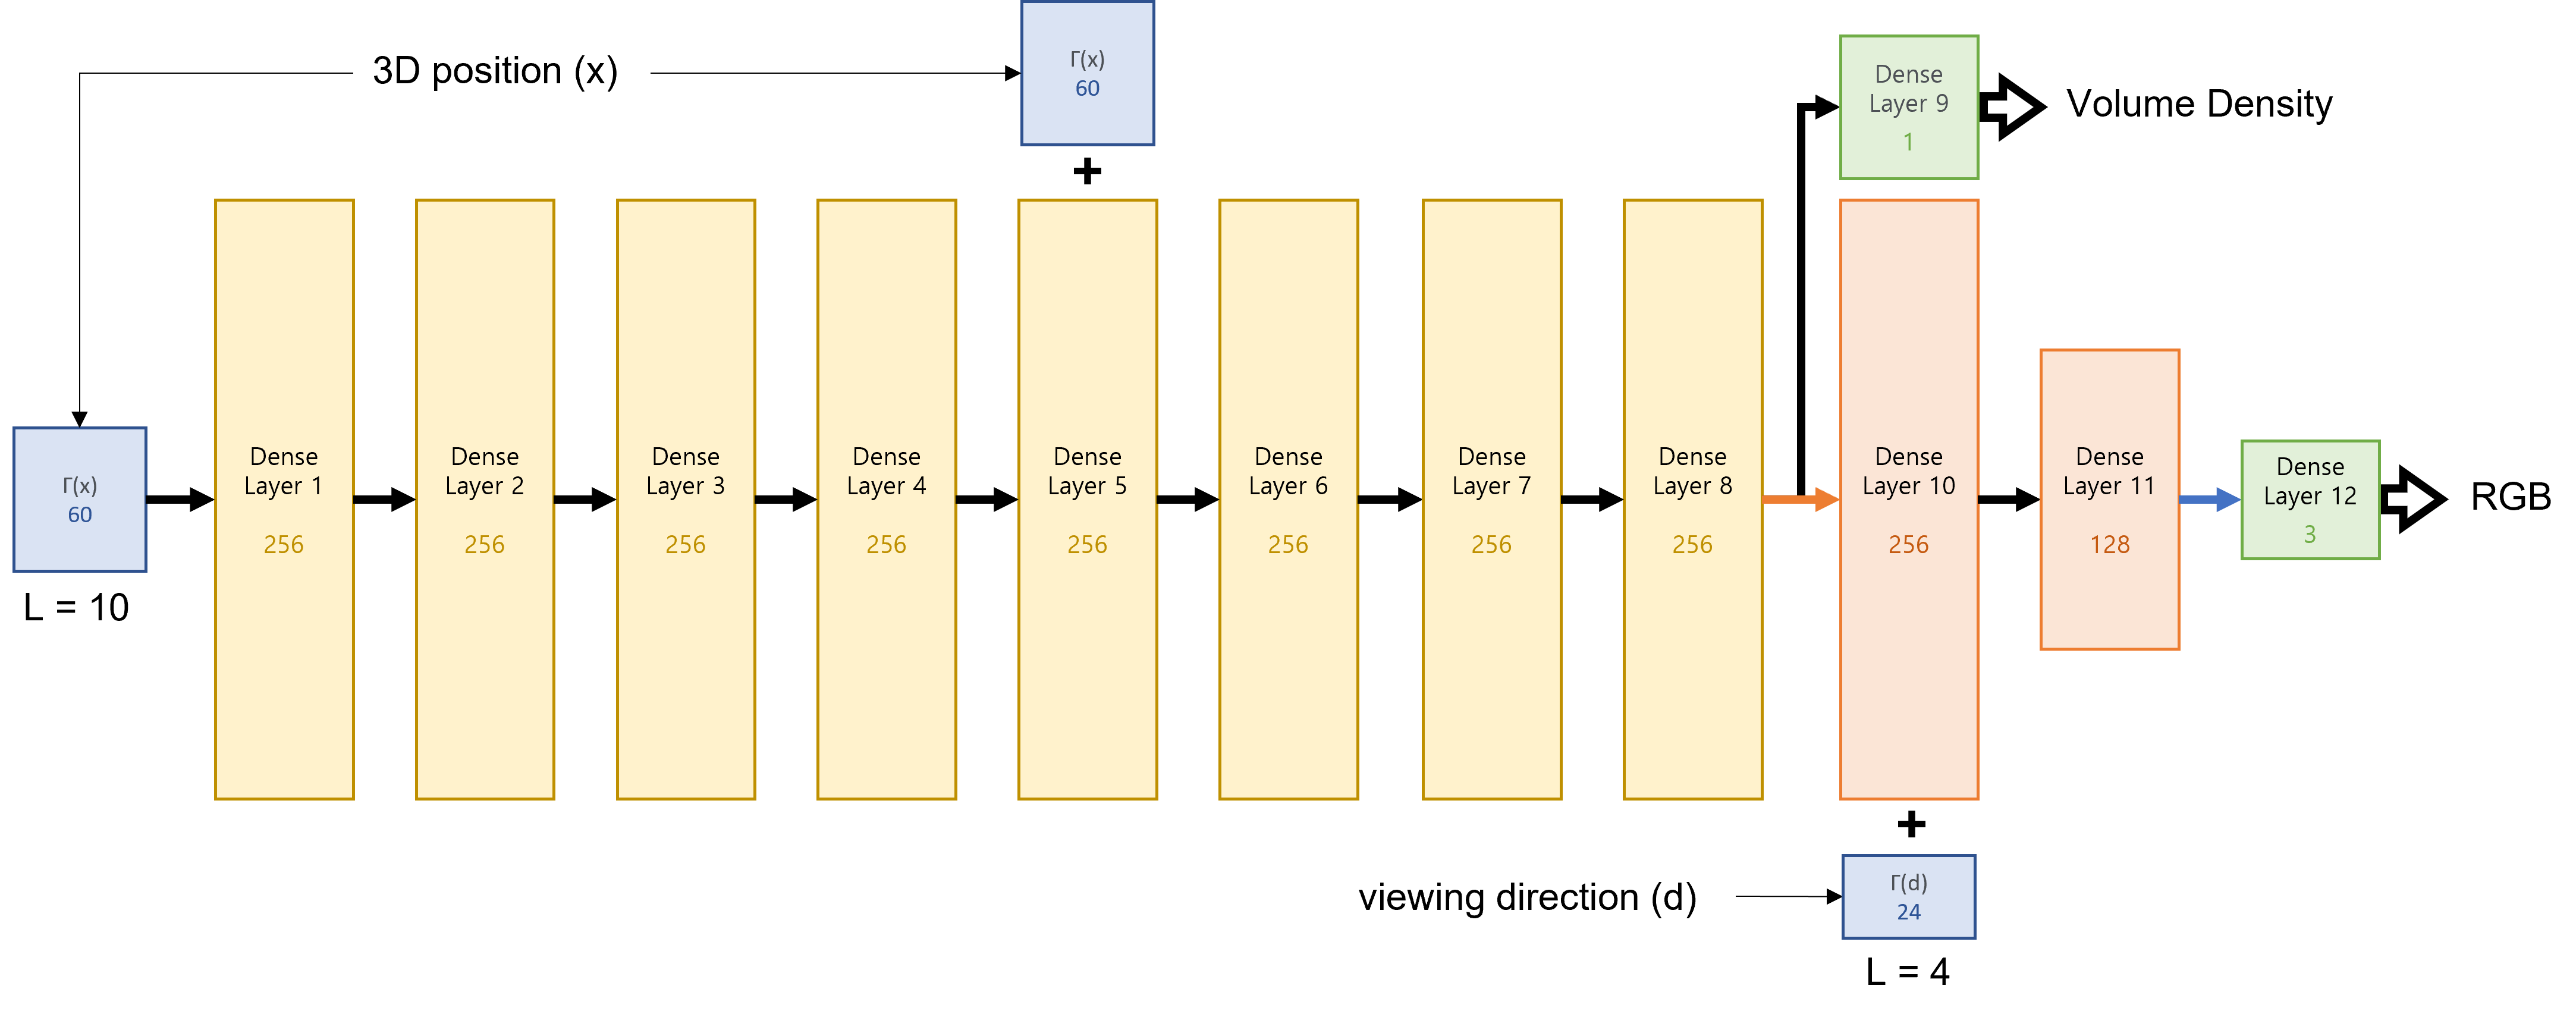
\includegraphics[width=0.9\textwidth]{../images/230710/NeRF_MLP.png}}\hfill
    \caption{Query into MLP ($x , y , z , \theta ,\phi $)}
    \label{fig:network}
\end{figure}

% Figure \ref{fig:network} ~~ 

왜 저러한 구조를 만들었는지는 실험은 통한 결과일 것으로 생각된다. 


\section{infoNeRF\cite{infonerf} reproduce}

\subsection{실험 데이터} 

코드와 함께 제공된 데이터를 이용하여 논문의 결과를 reproduce 하였다. 

\subsection{reproduce 결과}

\begin{figure}[h]
    \centering
    \subfloat[GT scene]{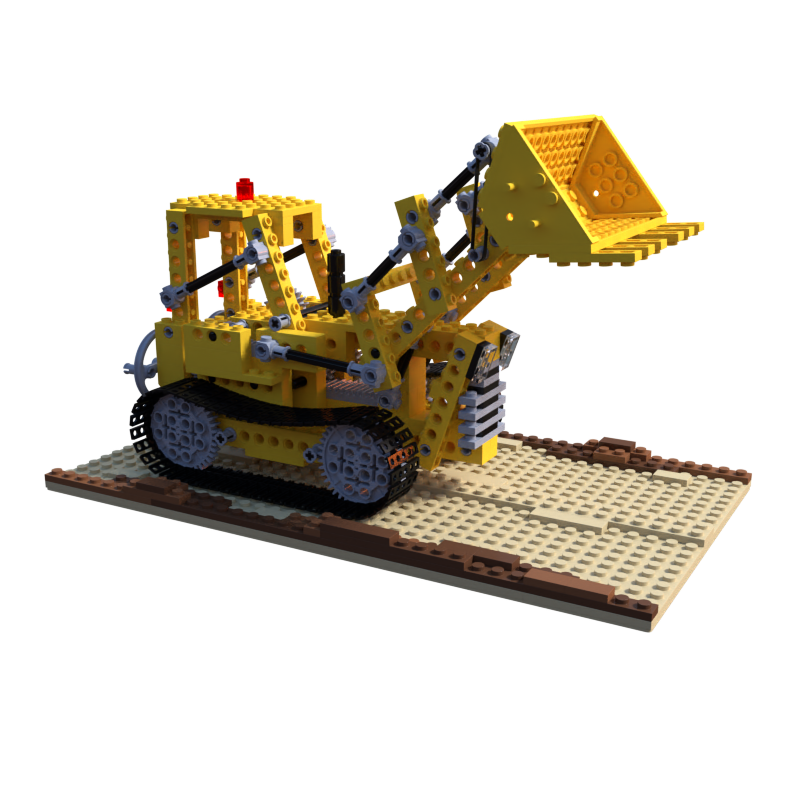
\includegraphics[width=0.3\textwidth]{../images/230710/GT.png}}\hfill\\
    
    \subfloat[NeRF 6000iter]{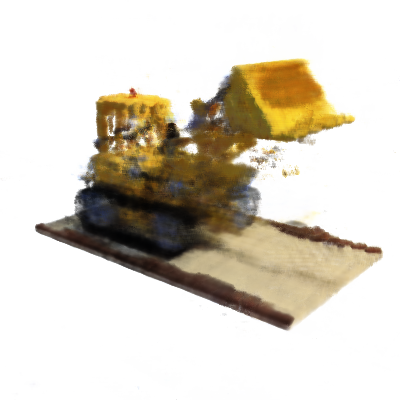
\includegraphics[width=0.3\textwidth]{../images/230710/NeRF_6000_017.png}}\hfill
    \subfloat[NeRF 48000iter]{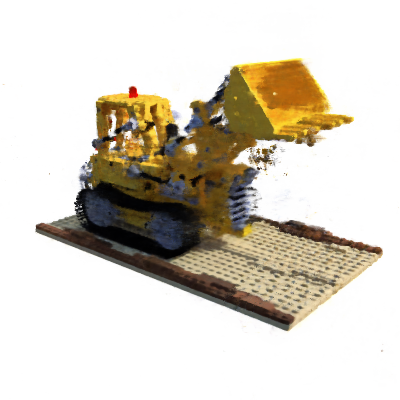
\includegraphics[width=0.3\textwidth]{../images/230710/NeRF_48000_017.png}}\hfill
    \subfloat[NeRF 48000iter]{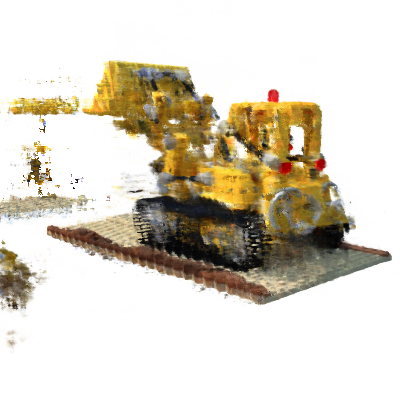
\includegraphics[width=0.3\textwidth]{../images/230710/NeRF_48000_011.png}}\hfill

    \subfloat[infoNeRF 6000iter]{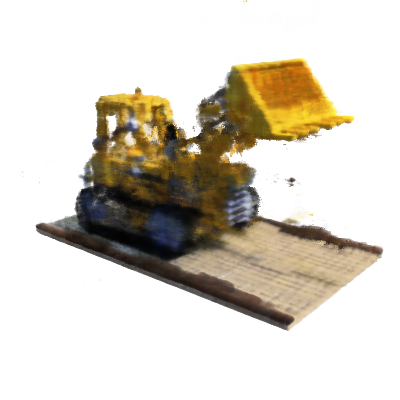
\includegraphics[width=0.3\textwidth]{../images/230710/infonerf_6000_017.png}}\hfill
    \subfloat[infoNeRF 48000iter]{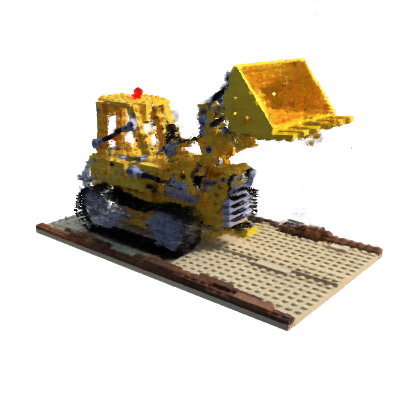
\includegraphics[width=0.3\textwidth]{../images/230710/infonerf_48000_017.png}}\hfill
    \subfloat[infoNeRF 48000iter]{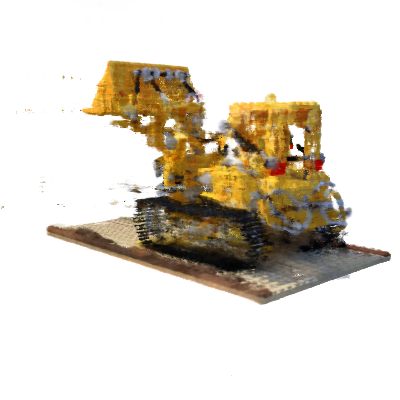
\includegraphics[width=0.3\textwidth]{../images/230710/infonerf_48000_011.png}}\hfill

    \caption{Result of NeRF and infoNeRF(4 views , half resolution)}
    \label{fig:nerf_infoNeRF_compare}
\end{figure}

Figure\ref{fig:nerf_infoNeRF_compare}로부터 알 수 있듯이 6000,48000 Iteration 모두 infoNeRF가 더욱 좋은 성능을 보인다.
특히 (d)의 경우 이상한 위치에 point cluster가 생긴것 또한 확인이 가능하다.
논문에 의하면 5000 Iteration에 PSNR 20과 유사한 결과가 나왔지만 half resolution option을 
사용해서 인지 더욱 높은 25 정도의 PSNR 결과값를 얻을 수 있었다.



\section{Camera parameter(colmap)}

\subsection{colmap option 분석} 


colmap이 camera calibration을 위해 제공하는 option은 다음과 같다.


\begin{itemize}
    \item (single)pinhole : 카메라에 왜곡이 없을 경우 사용한다. 따라서 focal length와 extrinsic 정보를 반환한다.(*single 옵션은 x,y focal length가 일치하면 사용한다)
    \item (single)radial : 이미지의 렌즈 왜곡을 고려한다. K값을 추가적으로 반환해주며, 이러한 값을 이용하여 더욱 정교한 왜곡 보정이 가능해진다.(*single 옵션은 x,y focal length가 일치하면 사용한다)
    \item ext : opencv, fisheye등 intrinsic을 사전에 아는 경우 혹은 광각 카메라의 경우를 가정한 추가적인 option이 존재한다. 더욱 많은 k값을 사용한다.
\end{itemize}

실제 pinhole 카메라는 이론과 다르게 작은 볼록렌즈를 사용하여 빛을 받는 양을 늘린다. 
결국 렌즈가 추가되기 때문에 이제 distortion이 발생하기 시작한다. 
일반적인 노트북에 내장된 카메라가 이에 해당된다고 알고있다.이러한 특징 떄문인지
calibration option을 pinhole로 하여도 왜곡을 보정하기 위한 파라미터를 추정하려고 한다고 한다.
infoNeRF에 파라미터 파일을 참고하여 보면 카메라 파라미터 관련 정보로 camera angle x, rotation, transform matrix값을 사용한다. 
하지만 custom image의 경우 파라미터가 달라진다. 
아이폰을 사용하여 찍은 영상이기 떄문에 radial 옵션을 사용하는 것이 가장 정확한 카메라 파라미터를 찾을 수 있지만
NeRF 및 info NeRF 모델은 simple pinhole 옵션을 가정하는 것이 가장 적합하다고 생각된다. 
따라서 모델 학습을 위해서는 simple pinhole 옵션을 이용하여 카메라 파라미터를 찾거나, 모델의 rendering code를 
수정하여야 한다.



\subsection{colmap 실습} 

\begin{figure}[h]
    \centering
    \subfloat[camera extrinsic]{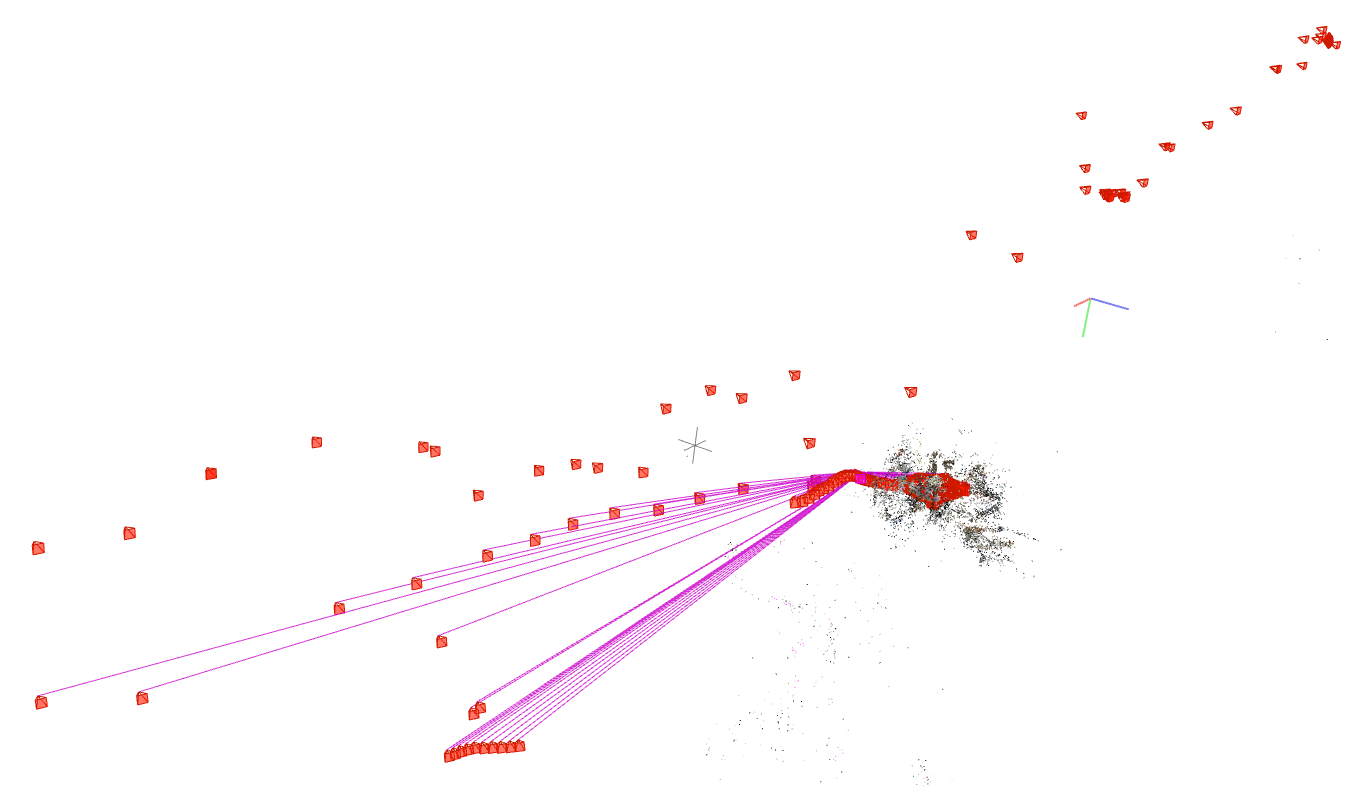
\includegraphics[width=0.6\textwidth]{../images/230710/colmap_error.png}}\hfill
    \subfloat[found features]{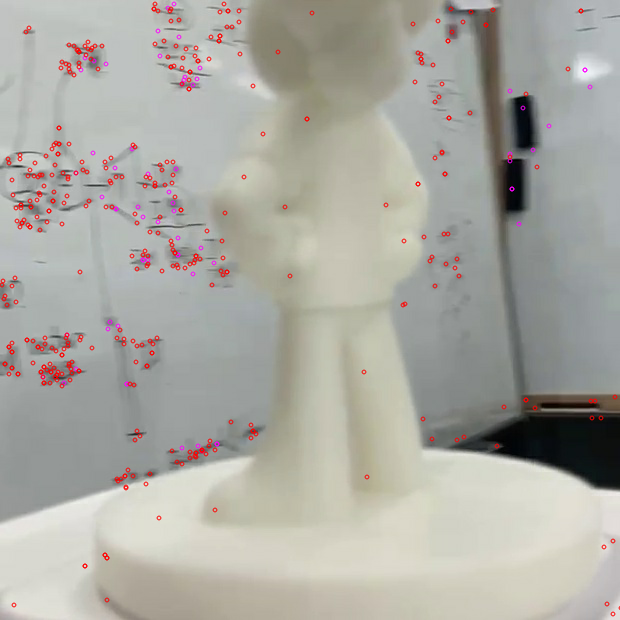
\includegraphics[width=0.4\textwidth]{../images/230710/colmap_sample.png}}\hfill
    \caption{colmap result}
    \label{fig:colmap_error}
\end{figure}

모델 학습을 위해 center crop 한 영상을 이용하여 simple pinhole을 통한 파라미터를 찾으려는 시도를 하였으나, 
colmap이 카메라 파라미터를 찾지 못하는 문제가 발생한다. 해당 이유로는 3가지를 생각해 볼 수 있다.

% \begin{figure}[H]
%     \centering
%     \subfloat{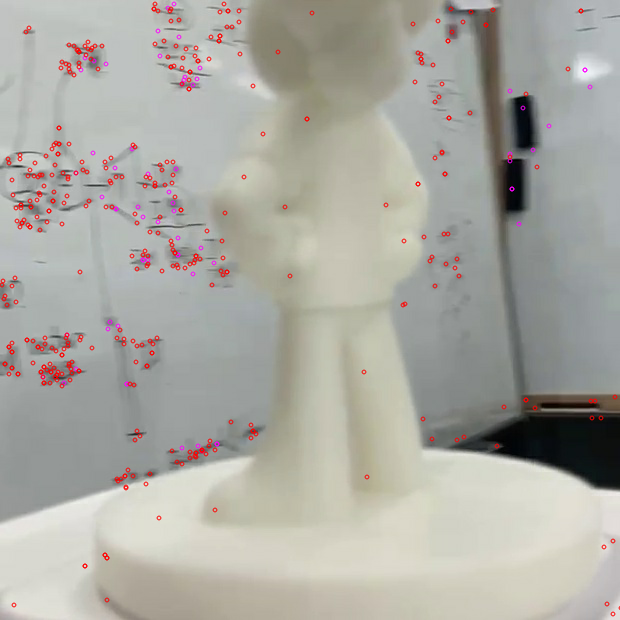
\includegraphics[width=0.4\textwidth]{../images/230710/colmap_sample.png}}\hfill
%     \caption{colmap feature extraction}
%     \label{fig:colmap_sample}
% \end{figure}

\begin{itemize}
    \item 해당 방법은 이미지 중앙은 왜곡이 없을 것을 가정하지만 실제로는 그렇지 않다.
    \item 아이폰 카메라가 별도의 추가적인 post processing을 진행하거나 조리개, 초점등 값이 매 frame 변화하며 오차가 발생한다.(auto focus 기능을 꺼야한다)
    \item \ref{fig:colmap_error}에서 colmap이 찾은 Feature는 물체보다 배경의 feature를 주로 찾은 것을 확인 가능하다. 물체에 360도 영상을 찍었지만 배경 feature를 사용하여 카메라 파라미터를 추론 중이다.
\end{itemize}


\section*{Action items in next week}	%% Action items in next week
다음 주에는 
\begin{enumerate}
    \item NeRF, infoNeRF 추가학습
    \item custom data를 통한 infoNeRF 실험 
\end{enumerate}
등을 진행하도록 하겠습니다.


\bibliographystyle{IEEEtran} 
\bibliography{refer} 
\end{document}